\section{Theorie}
\label{sec:Theorie}

Es ist bekannt, dass bewegte elektrische Ladungen magnetische Felder erzeugen (z.B. ein bewegtes Elektron).
Dabei lässt sich das Magnetfeld als eine Vektorgröße beschreiben, dessen Richtung und Betrag durch die magnetische Feldstärke $\vec{H}$ beschrieben wird.
Die magnetische Flussdichte wird beschrieben durch

\begin{equation} \label{eq:Flussdichte}
    \vec{B} = \mu \vec{H} = \vec{B} = \mu_{0} \mu_{r} \vec{H}
\end{equation}

wobei $\mu$ die \textit{Permeabitlität}, $\mu_{0}$ die \textit{Vakuum-Permeabitlität} und $\mu_{r}$ die \textit{relative Permeabitlität} ist.
FÜr bewegte Ladungen in einem stromdurchflossenen Leiter gilt das \textit{Biot-Savartsche Gesetz:}

\begin{equation} \label{eq:Biot-Savart-Gesetz}
    \vec{B}(\vec{r}) = \frac{\mu_{0}I}{4pi} \int \frac{d\vec{s} \times \vec{r}}{r^3}
\end{equation}


\begin{minipage}{0.7\textwidth}
    Dabei beschreibt $I$ den Strom, der durch gegebenen Leiter fließt und $d\vec{s}$ das Leiterstück.
\end{minipage}
\begin{minipage}{0.3\textwidth}
    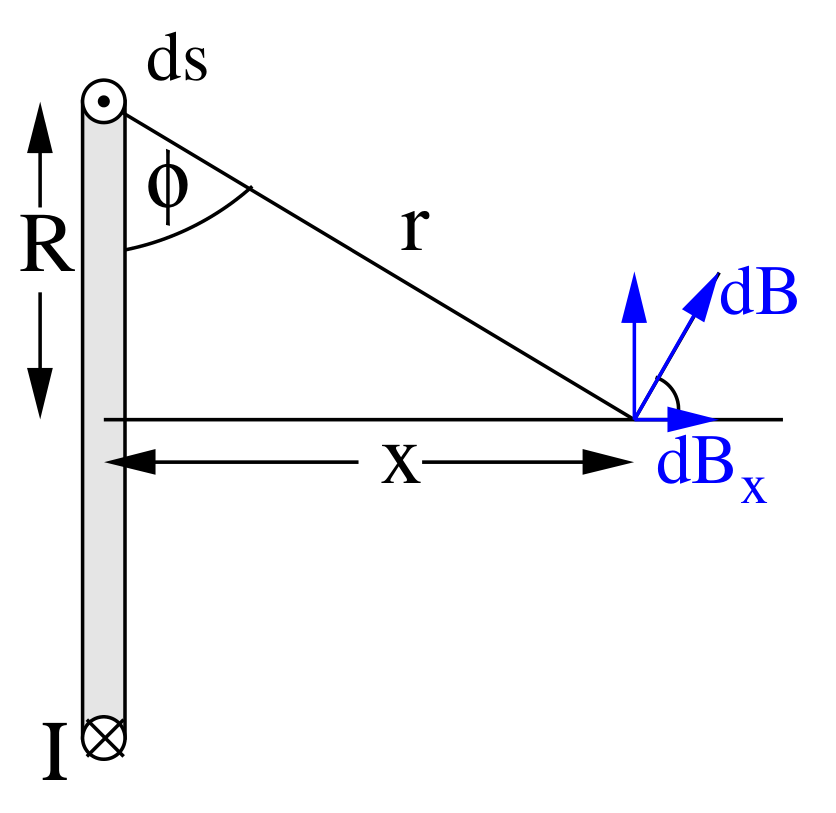
\includegraphics[width=\textwidth]{pictures/BiotSavart1.png}
\end{minipage}

Durch die Gleichung (\ref{eq:Biot-Savart-Gesetz}) ergiebt sich die wichtige Formel für Leiterschleifen.

\begin{equation} \label{eq:Leiterschleife}
    \vec{B}(x) = \frac{\mu_{0}I}{2} \frac{R^2}{(R^2 + x^2)^{3/2}} \frac{\vec{x}}{|x|}
\end{equation}

Nun ist innerhalb stromdurchflossenen Spulen das Magnetfeld annähernd homogen und die Gleichung (\ref{eq:Leiterschleife}) bedarf einer Anpassung.
Denn wir haben nun $N$ Windungen und die Spule eine Länge $l$:

\begin{equation} \label{eq:LangeSpule}
    B = \mu_{0}\mu_{r}I \frac{N}{l}
\end{equation}

Dabei ist zu beachten, dass diese Gleichung ihre Gültigkeit außerhalb der Spule verliert, da das Magnetfeld dort inhomogen wird.

Das Magnetfeld der Ringspule lässt sich ebenfalls über das Bio-Savart Gesetz (\ref{eq:Biot-Savart-Gesetz}) berechnen.
Die Ringspule ist charakterisiert durch die Windungszahl $N$ und den Radius $R$.
Man kommt schließlich auf folgende Gleichung:

\begin{equation}
    B = \mu_{0}\mu_{r}I \frac{N}{2\pi R}
\end{equation}

Das Magnetfeld eines Helmholtzspulenpaares, zwei identische Spulen im Abstand $x$ zum Mittelpunkt, berechnet sich wie folgt:

\begin{equation}
    B(0) =  B_{1}(x) +  B_{1}(-x) = \frac {\mu_{0} I R^2} {(R^2 + x^2)^{3/2}}
\end{equation}